The equations of planes are
\begin{align}
    &p_1:\vec{{n_1}}^Tx=1\\
    &p_2:\vec{{n_2}}^Tx=-4
\end{align}
where
\begin{align}
    &\vec{n_1}=\myvec{1 & 1 & 1}^T \label{sep/2/40/eq:eq1}\\
    &\vec{n_2}=\myvec{2 & 3 & -1}^T \label{sep/2/40/eq:eq2}
\end{align}
The equation of the desired plane is given by
%
\begin{align}
    & (\vec{n_2}+\lambda \vec{n_1})^T\vec{x}=d_2+\lambda d_1
\end{align}
Since the plane is parallel to x-axis,
\begin{align}
  & \vec{e_1}^T(\vec{n_2}+\lambda \vec{n_1})=0\\
    \implies &\lambda=-2
\end{align}
The required plane is given by
\begin{align}
    &(\vec{n_2}-2\vec{n_1})^T \vec{x}=d_2-2d_1\\
    &\myvec{0 & 1 & -3}\vec{x}=-6
\end{align}
    
A plot for the planes is given in Fig.     \ref{sep/2/40/plot}.

\begin{figure}[!ht]
    \centering
    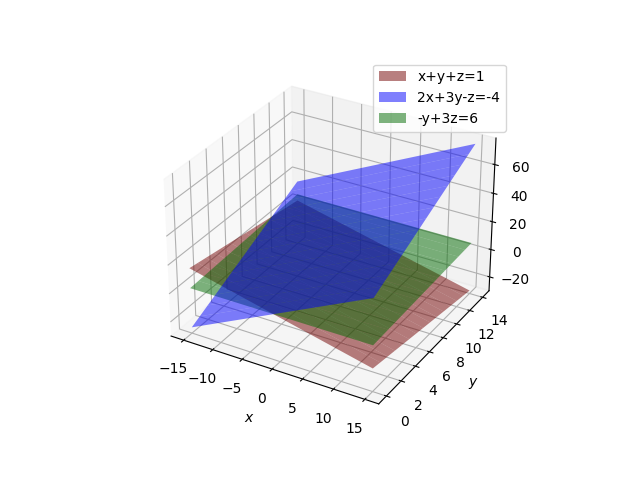
\includegraphics[width=\columnwidth]{solutions/sep/2/40/plot/Figure_1.png}
    \caption{Plot of the planes}
    \label{sep/2/40/plot}
    \end{figure}
